\section{実験結果と考察}
基準AによるBの校正時のドリフト測定の結果を図\ref{fig:ドリフト1}に示す.変位計Aの変位は負の方向に傾くように変化したが,変位計Bはほとんど変位していなかった.
基準BによるAの校正時のドリフト測定の結果を図\ref{fig:ドリフト2}に示す.変位計Aは変位0.060mm/divでほぼ一定だったが,変位計Bは負の方向に傾くようなグラフとなった.

\begin{figure}[htbp]
    \centering %中央揃え
    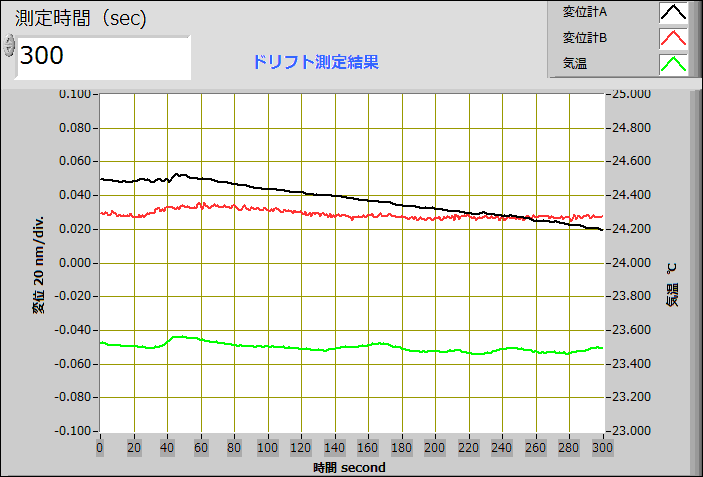
\includegraphics[width=100truemm,clip]{fig/温度ドリフト測定結果(Step1前)_A.png}
    \caption{Temperature drift measurement results(Calibration of B with reference A).}
    \label{fig:ドリフト1}
\end{figure}
\begin{figure}[htbp]
    \centering %中央揃え
    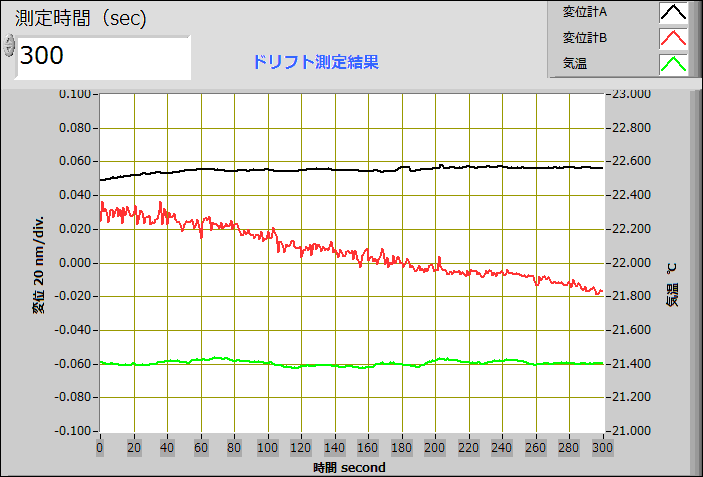
\includegraphics[width=100truemm,clip]{fig/温度ドリフト測定結果(Step2前)_A.png}
    \caption{Temperature drift measurement results(Calibration of A with reference B).}
    \label{fig:ドリフト2}
\end{figure}

図\ref{fig:測定結果}に測定した校正曲線と室温のグラフを示す.図\ref{fig:演算結果}には,演算により得られた校正曲線と線形誤差のグラフを示す.線形誤差は演算の度に変化が小さくなるためグラフが重なっており,5回目の結果のみが見られる.
\begin{figure}[htbp]
    \centering %中央揃え
    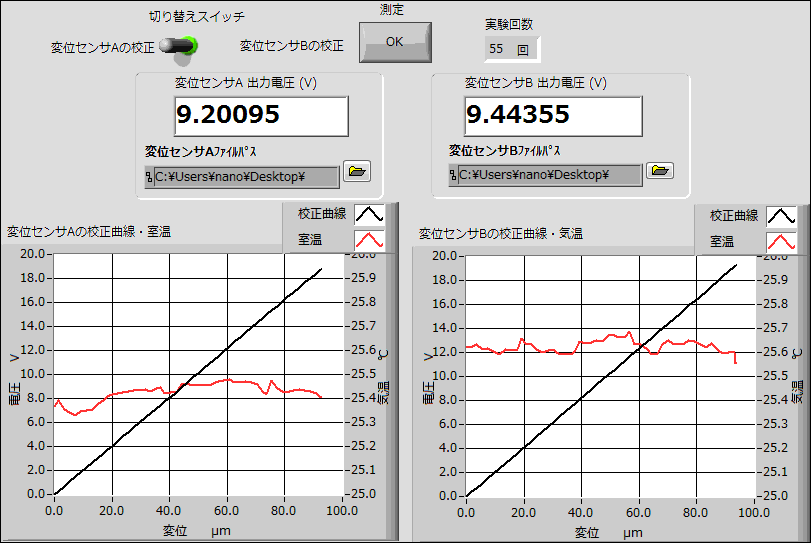
\includegraphics[width=100truemm,clip]{fig/測定結果_D.png}
    \caption{Calibration curve and room temperature measurement results.}
    \label{fig:測定結果}
\end{figure}
\begin{figure}[htbp]
    \centering %中央揃え
    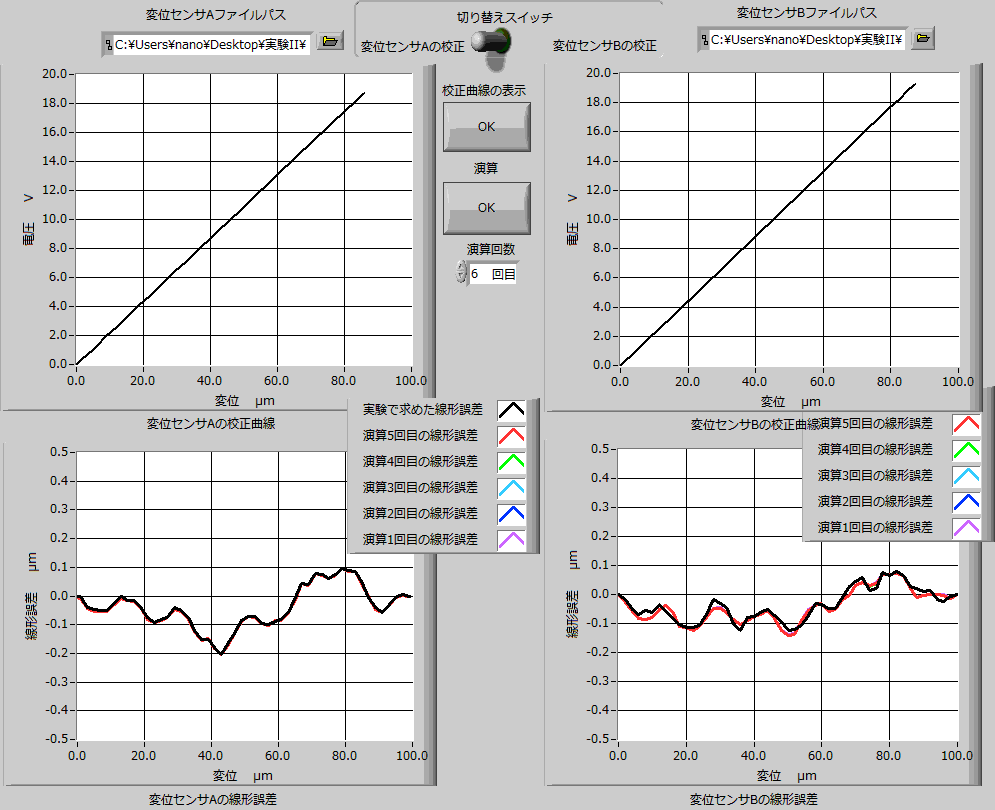
\includegraphics[width=100truemm,clip]{fig/演算結果_A.png}
    \caption{Graphs of calibration curves and their linear errors due to arithmetic operations.}
    \label{fig:演算結果}
\end{figure}